% !TEX encoding = UTF-8 Unicode
\documentclass[a4paper]{article}

\usepackage[utf8]{inputenc}
\usepackage{erk}
\usepackage{times}
\usepackage{graphicx}
\usepackage[top=22.5mm, bottom=22.5mm, left=22.5mm, right=22.5mm]{geometry}

\usepackage[slovene,english]{babel}

% local definitions
\def\footnotemark{}%  to avoid footnote on cover page

\begin{document}
%make title
\title{WSN(BSO) final report}

\author{Denis Vitez$^{1}$, Luka Golinar$^{1}$} % use ^1, ^2 for author(s) from different institutions

\affiliation{$^{1}$University of Ljubljana, FRI}

\email{E-mail: dv9763@student.uni-lj.si, lg7681@student.uni-lj.si}

\maketitle

%\thispagestyle{empty}

\begin{abstract}{Abstract}
This paper will present the finding and results of a final seminar project at subject WSN (Wireless sensor networks).
\end{abstract}


\selectlanguage{english}

\section{Problem}
The problem that we had to tackle in the seminar project was to develop an wireless sensor network, that will use physical Zolertia Z1 motes and also virtual motes inside Cooja program that is bundled with the Contiki operating system, that was running on our devices. The resulting network had to be robust, so it would handle failure of one or multiple motes and also the requirement for the network had to use multihop, since not all nodes were in direct range with one another. After the network has been setup, we had to implemented differenc actions that the network could perform. For example network had to return results for given queries (temperature, vibration level, ...). The other requirement was for the network to be able to detect anomalies and report them to the "master" node.
\section{Design}
For our system framework, we used the existing ipv6 udp example provided by contiki. We decided to use UDP instead of rime, as we tought it provided a more simplistic implementation of multicast and it did mostly what we wanted it to do. We categorized our design in a few key aspects. The system should be able to auto-detect mote failure, it should be able to report sensors values both on demand and automtically in case a certain threshold is hit and it should be as power eficient as possible.

We implemented te design using Cooja, a tool avaliable in the InstantContiki OS. This provided us with a simulation environment when different scenarios could be tested. Our project should include two types of motes:
\begin{itemize}
\item Virtual motes
\item Physical motes
\end{itemize}
Virtual motes are divided by their function:
\begin{itemize}
\item Root mote
\item Sink mote
\item Gateway sink
\end{itemize}
The root motes servers as a master mote. This mote is directly connected to a power source and easily accessible. We assumed therefore, that this mote can not fail. It is the task of the root mote to directly accept user input commands, which are issued directly via serial port, using the UART protocol. The root mote then sends a broadcast message to all avaliable motes, which have connected to the multicast network. The root mote is also in charge of storing and printing all the sensor data collected through the network.

Sink motes are basically child motes. These motes have the task to report their sensor data and forward data directed to the root mote. There is a variety of different sensors avaliable to the Zolertia modules, but we've only implemented acquisition of temperature and vibration sensors. Our project supports minimum, maximum and average values across all the network.

These is also a special type of sink mote, which is called a gateway sink. The job for this mote is to redirect all commands received from the root mote to phyisical motes. The main physical mote is called re\_gateway\_root. It's job is basically the same as the root virtual mote, except all the data is relayed back to the serial port, where the gateway sink can intercept it and send it back to the virtual root mote. To achieve this connection, we've used serial2usb plugin, provided on ucilnica. This plugin allows a certain virtual mote to send data directly to a pts device. We then used a multipurpose relay tool called socat, to connected the root pts device with a USB device (typically this would be /dev/ttyUSB0), where our physical root mote is connected to. This way, we basically have two multicast networks, one virtual and one real.
\newline
\newline

\section{Implementation}
\subsection{Routing}
Our design uses UDP for communication. Our root is the UDP server, and sinks are clients. The server does three tasks primarily.

\begin{itemize}
\item Initializes RPL DAG
\item Setup up UDP connections
\item Waits for packes from clients 
\end{itemize}

Packets are processed using the tcpip\_handler function, which was already provided by Contiki. We've modified this function for our own needs. All the motes have the tcpip\_handler function, since our network also supports queries and both the root mote and sink motes should be able to receive and send packets.

\subsection{Commands}
Commands are issued in SCPI - 99 compliant standard. They are represented with the following structure: \textbf{NETWORK:FAMILY:FUNCTION:PART}.
\begin{figure}[!htb]
    \begin{center}
        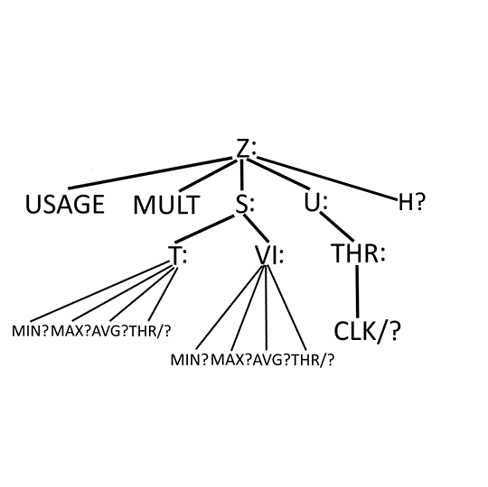
\includegraphics[scale=0.8]{structure.png}
        \caption{Tree structure of messages.} \label{pic1}
    \end{center}
\end{figure}

In out assignment we had to support the following queries (Q) and alarms (A):
\begin{itemize}
\item \textbf{Q:} Maximum temperature across the whole network.
\item \textbf{Q:} Minimum temperature across the whole network.
\item \textbf{Q:} Find nodes with maximum vibration level.
\item \textbf{Q:} Average vibration level across the whole network.
\item \textbf{Q:} Find currently connected nodes (heartbeat).
\item \textbf{A:} Report if temperature at some sensor exceeds a certain threshold.
\item \textbf{A:} Report if vibration at some sensor exceeds a certain threshold.
\end{itemize}
\section{Optimization}
\subsection{Power consumption}
\subsection{Memory usage}
\section{Results}
Results and graphs from Cooja should go here...
\section{Problems}
\section{Conclusion}
\small
\begin{thebibliography}{1}

\bibitem{ERK} ERK, http://www.ieee.si/erk/index.html 
\bibitem{Zbornik} B. Zajc, A. Trost: Zbornik triindvajsete mednarodne Elektrotehniške in računalniške konference ERK 2014, 22. - 24. September 2014, Portorož, Slovenija

\end{thebibliography}

\end{document}
